\chapter{Flujos de trabajo}
\label{chap:workflows}

\section{Definición y ejemplos}
Un flujo de trabajo es un conjunto de pasos que modelan la ejecución de un proceso \cite{gutierrez2012agent}.
%En la literatura especializada, los flujos de trabajos también son conocidos como \emph{workflows}.%
En particular, en esta tesis se estudian a los flujos de trabajo utilizados para vislumbrar la ejecución de un proceso de cómputo. A continuación, se muestran algunos ejemplos de estos flujos de trabajo.

\subsection{Anotación de proteínas}
En el proyecto \emph{e-Protein}, realizado por la Escuela Imperial de Londres, se realizó un flujo de trabajo para la anotación de proteínas. El objetivo del proyecto \cite{o2004mapping} era la identificación y anotación de partes de proteínas que expliquen su estructura y su función. En la figura \ref{fig:iceni-workflow} se muestra el flujo de trabajo desarrollado, donde las cajas representan los programas que son ejecutados para cada paso del proceso de anotación, y las líneas que conectan a las cajas representan las dependencias de datos entre los programas, es decir, si una caja tiene una línea que apunta a ella, significa que dicho programa depende de otro programa determinado por el otro extremo de la flecha.

\begin{figure}
\begin{center}
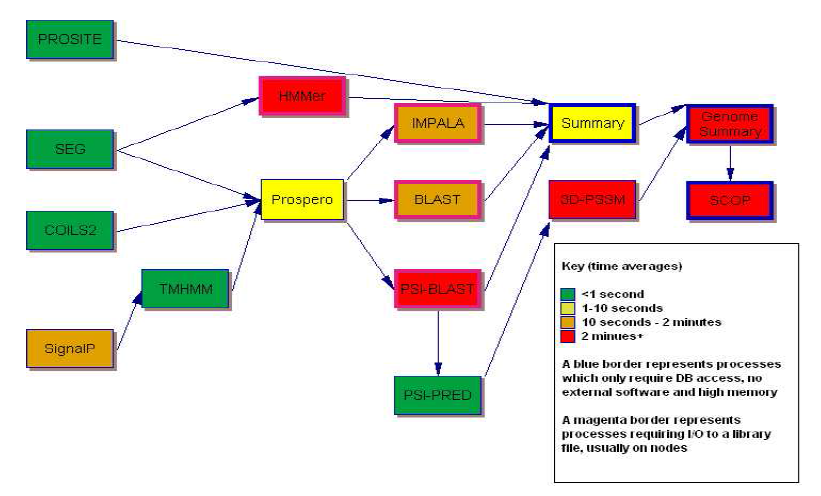
\includegraphics[width=0.8\textwidth]{imagenes/iceni-workflow}
\end{center}
\caption{Flujo de trabajo para la anotación de proteínas.}
\label{fig:iceni-workflow}
%diseñado en la Escuela Imperial de Londres para el proyecto \emph{e-Protein}.
\end{figure}


\subsection{Curvas de amenaza sísmica}
Otro notable ejemplo es el proceso para generar curvas de amenaza sísmica que describen las probabilidades de que ocurra un temblor en una determinada área. Para elaborar estas curvas, los científicos del Centro de Terremotos del Sur de California (SCEC por sus siglas en inglés) tienen que realizar una gran cantidad de simulaciones para que sus resultados puedan ser combinados y expresados en la curva de amenaza \cite{deelman2006managing}. El flujo de trabajo para generar la curva de amenaza se muestra en la figura \ref{fig:scec-workflow}.

\begin{figure}
    \begin{center}
        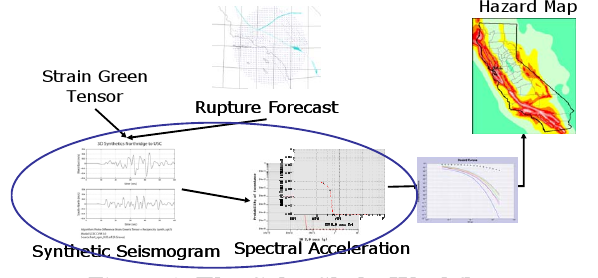
\includegraphics[width=0.8\textwidth]{imagenes/scec-workflow}
    \end{center}
    \caption{Flujo de trabajo para generar curvas de amenaza sísmica.}
    %elaborado por el SCEC
    \label{fig:scec-workflow}
\end{figure}

\subsection{Generación de facturas}
Recientemente en México, el Sistema de Administración Tributaria emitió los lineamientos para que las operaciones de compra-venta entre personas físicas y morales puedan ser registradas por medio de facturas electrónicas. Para generar estos Comprobantes Fiscales Digitales, las empresas tienen que hacer procesos de validaciones de RFC y encriptar el contenido de la factura con un mecanismo de llave privada. Naturalmente, este proceso de generación de facturas requiere de varias actividades. En la figura \ref{fig:cfd-workflow} se muestra el flujo de trabajo que utiliza una empresa para generar sus facturas. Este flujo se encuentra documentado en una tesina presentada por Alcerreca \cite{alcerreca2013cfd}.

\begin{figure}
    \begin{center}
        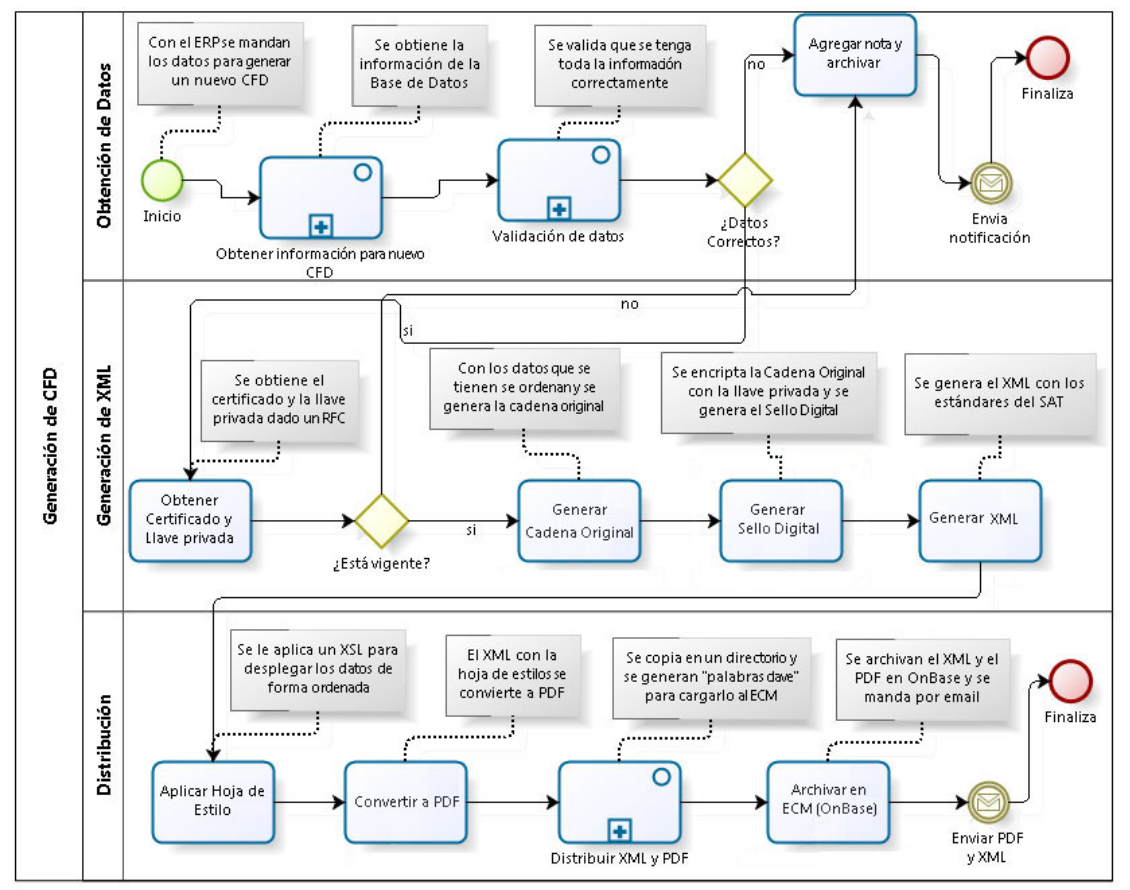
\includegraphics[width=0.8\textwidth]{imagenes/cfd-workflow}
    \end{center}
    \caption{Flujo de trabajo para generar facturas electrónicas.}
    %utilizado por una empresa de cementos
    \label{fig:cfd-workflow}
\end{figure}

\subsection{Procesamiento de imágenes astronómicas}

La NASA elaboró un software que permite crear una gran imagen del espacio exterior a partir de varias imágenes mosaico tomadas desde distintos telescopios. Esta aplicación, llamada Montage, utiliza un flujo de trabajo para generar la gran imagen. En la fase inicial de procesamiento, cada una de las imágenes mosaico puede ser procesada de manera independiente. En la figura \ref{fig:montage-workflow} se puede observar que el flujo de trabajo del proyecto Montage inicia con varias actividades en paralelo, donde el color de las actividades representan la fase de procesamiento de la imagen. Luego, en la actividad de color gris, todas las imágenes son juntadas para generar la imagen de fondo común para todas las imágenes mosaico.

\begin{figure}
    \begin{center}
        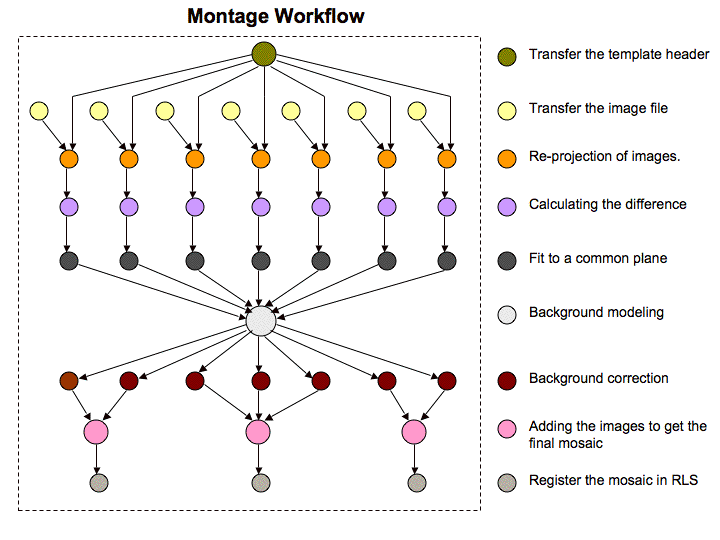
\includegraphics[width=0.8\textwidth]{imagenes/montage-workflow}
    \end{center}
    \caption{Flujo de trabajo para procesar imágenes del proyecto Montage.}
    %utilizado por una empresa de cementos
    \label{fig:montage-workflow}
\end{figure}



\section{Estructura de los flujos de trabajo}
\label{secc:workflow_str}
Como hemos visto en los tres ejemplos anteriores, los flujos de trabajo presentados describen los \emph{pasos} que se necesitan para calcular la solución de un problema. En éstos, no se ha hablado sobre los detalles para hacer los cómputos necesarios para cada flujo. En los flujos de trabajo tampoco se han definido las plataformas de cómputo en que se ejecutan estos flujos. Tan sólo se han definido los grandes pasos para solucionar el problema y las dependencias que tienen estos pasos. 

Ahora, es muy común que estas dependencias estén dictadas por los datos que requiere cada paso para funcionar. Sin embargo, hay situaciones en los que los pasos del flujo no requieren los datos del paso anterior para funcionar, sino que las dependencias están marcadas por el orden temporal que deben seguir estos pasos. Así, se puede notar una ambigüedad en la definición de un flujo de trabajo.

\section{Perspectivas de los flujos de trabajo}
En la sección \ref{secc:workflow_str} se argumentó que un flujo de trabajo puede representar varias cosas, a saber: el orden temporal de las tareas o las dependencias de datos entre cada tarea, produciendo una ambigüedad en la interpretación de un flujo de trabajo. Debido a esta ambigüedad del significado de un flujo de trabajo, es posible interpretar un flujo de trabajo desde varias perspectivas. En el trabajo de Van der Aalst et al. \cite{van2003workflow} se identifican una serie de perspectivas identificadas en las definiciones de las especificaciones de un flujo de trabajo utilizadas en los sistemas que administran la ejecución de flujos de trabajo. Las cuatro perspectivas se enuncian a continuación:
%En esta tesis, tomaremos estas perspectivas a manera de una clasificación de flujos de trabajo basadas en la forma en que describen sus dependencias

\begin{itemize}
\item{\textbf{Perspectiva de control de flujo.} Describe las relaciones de las actividades (pasos) con estructuras de control, tales como: secuencia, decisión, ejecución de actividades en paralelo y punto de sincronización conjunta. El flujo de trabajo para la generación de facturas es un buen ejemplo de un flujo de trabajo visto desde la perspectiva de control de flujo porque, al observar la figura \ref{fig:cfd-workflow}, se pueden notar que hay actividades, simbolizadas con un rombo, que determinan si se ejecutan o no ciertas tareas.
%\footnote{Esta estructura de control también es conocida como \emph{join synchronization}}.
}

\item{\textbf{Perspectiva de datos.} En ella, los flujos de trabajo describen las entradas y salidas de datos, tanto de ejecución como de control, que se tienen en cada actividad del flujo. También se toman en cuenta los datos locales a cada actividad; es decir, que sólo son necesarios dentro del contexto de ésta. En el ejemplo del flujo de trabajo para la anotación de proteínas, mostrado en la figura \ref{fig:iceni-workflow}, podemos ver que esta perspectiva describe adecuadamente la estructura del flujo, ya que el orden de ejecución de las actividades están definidas por los datos que requieren cada una de las actividades.}

\item{\textbf{Perspectiva de recursos.} Muestra cuáles son los recursos con los que se cuentan para ejecutar el flujo de trabajo y la forma en que estos recursos se encuentran organizados. Estos recursos pueden ser desde entidades de cómputo hasta roles con responsabilidades específicas cumplidas por actores humanos. El flujo de trabajo para generar curvas de amenaza sísmica de la figura \ref{fig:scec-workflow} es un ejemplo de esta perspectiva, porque los elementos necesarios para generar las curvas de amenaza son provistos por geólogos.}

\item{\textbf{Perspectiva operacional.} Aquí se detallan las operaciones elementales necesarias en cada actividad para ejecutar el flujo de trabajo. Estos detalles incluyen las transferencias de datos entre las operaciones y su correspondencia en programas. El flujo de trabajo del proyecto Montage, mostrado en la figura \ref{fig:montage-workflow} ejemplifica esta perspectiva, ya que los colores utilizados en el flujo de trabajo son las actividades específicas que se aplican a cada imagen a procesar.}
\end{itemize}

Cabe aclarar que estas perspectivas están relacionadas entre sí de modo que el control de flujo es la base en la que descansan las demás perspectivas. Esto es porque la perspectiva de datos requiere que el control de flujo tenga los datos de entrada y salida como prueba de que se cumplieron las pre y post-condiciones de cada actividad, respectivamente; la perspectiva de recursos define con qué se ejecutarán y almacenarán los datos del flujo de trabajo; mientras que la perspectiva operacional trata los detalles sobre cómo se utilizan físicamente los recursos, los datos y los programas a lo largo del flujo de trabajo.


\section{Planificación como control de flujo}

El hecho de que la perspectiva de control de flujo sea la base de las demás perspectivas indica que la forma en que controla la ejecución del flujo determina de manera fundamental el rendimiento de la ejecución total de una instancia del flujo de trabajo. Por lo tanto, es de vital importancia encontrar métodos de planificación que permitan encontrar correspondencias entre recursos y actividades que cumplan con los requisitos dictados en las especificaciones examinadas en la perspectiva del control del flujo y que también maximicen el rendimiento de la ejecución de todo el flujo en general.

\section{Alcance}

En este trabajo, se establecerán las siguientes consideraciones para definir el alcance de este estudio de los algoritmos de planificación, a saber: la utilización de grafos dirigidos acíclicos y la suposición de que no habrá errores en la ejecución atómica de las tareas de los flujos de trabajo. En las siguientes se explicarán la importancia de estas suposiciones.

\subsection{Grafos dirigidos acíclicos}
Los flujos de trabajo están representados como \emph{grafos dirigidos acíclicos}, con el objetivo de simplificar el estudio. Se utilizan estos grafos porque son una estructura de datos que representa intuitivamente las dependencias entre tareas. Se requiere que estos grafos sean dirigidos porque esta característica representa el orden de ejecución de las tareas. Además, el hecho de que no existan ciclos en los grafos implica que no se necesita ningún mecanismo de control de flujo condicional; es decir, si la ejecución de las tareas de un flujo de trabajo dependiera de las salidas de otras tareas del flujo, no se podría saber apriori cuál es el orden de ejecución de las tareas, y los algoritmos de planificación tendrían que especular cuál sería el posible orden de ejecución.

\subsection{Ejecución atómica de tareas sin fallos}
Las tareas (o actividades) de los flujos de trabajo son consideradas \emph{atómicas}, i.e., una tarea no puede ejecutarse incompletamente ni incorrectamente. Algunos sistemas de administración de ejecución de flujos de trabajo tienen mecanismos para lidiar con estos errores, pero el estudio de éstos queda fuera del alcance de este trabajo, debido a la complejidad que representa diseñar e implementar sistemas distribuidos tolerantes a fallos. Un ejemplo de un sistema de administración de flujos de trabajo se encuentra en el trabajo de Kandaswamy et al. \cite{kandaswamy2008fault}, en el cual describe que utilizan sobreprovisionamiento de recursos y migración de recursos para mitigar las fallas.

%\item{La información de las \emph{demás perspectivas} puede ser requerida, dependiendo si el mecanismo de planificación lo considere necesario para tomar mejores decisiones con el fin de optimizar el tiempo total de ejecución o cumplir con algunos criterios establecidos en la definición del flujo de trabajo.}

%conclusiones:
% - representar como DAG's porque es sencillo y expresivo (balanceado)
% - tareas atómicas
% - la información de las demás perspectivas se puede requerir o no, dependiendo de como lo requiera el planificador.


%ejemplo: ICENI tiene partes paralelas, que no requieren de ciertos datos para operar
%ejemplo: Si hablas de orden,
%poner ejemplos donse se ejemplifique esta calendarización

%clasificados de acuerdo a dependencias (de orden, o de datos)


%clasificados de acuerdo a nivel de detalle (específico para cada plataforma)

%clasificados de acuerdo a instancias
% - pocas instancias, mucho tiempo de cómputo:
% - intensivos en instancias, pero cortos en ejecución:

%todos se pueden representar como Grafos Dirigidos Acíclicos

%implementaciones de representación de workflows
% - AGWL